% -*- coding: utf-8 -*-
\documentclass[12pt]{article}
\special{papersize=3in,5in}
\usepackage[utf8]{inputenc}
\usepackage{amssymb,amsmath}
\pagestyle{empty}
\setlength{\parindent}{0in}
\begin{document}

\begin{note}
    \xplain{Was ist ein Produkt?}
    \xplain{„Ein Produkt ist das Ergebnis einer Organisation, das ohne jegliche Transaktion zwischen Organisation und Kunden erzeugt werden kann.“ (ISO 9000:2015)}
\end{note}

\begin{note}
    \xplain{Was ist sind Anforderungen?}
    \xplain{„Anforderungen sind Erfordernisse oder Erwartungen, die festlegt, üblicherweise vorausgesetzt oder verpflichtend sind.“ (ISO 9000:2015)}
\end{note}

\begin{note}
    \xplain{Nenne Qualitätsmerkmale}

    \begin{field}
        \begin{itemize}
            \item Funktionalität
            \item Zuverlässigkeit
            \item Benutzbarkeit
            \item Effizienz
            \item Wartungsfreundlichkeit
            \item Übertragbarkeit
        \end{itemize}
    \end{field}
\end{note}

\begin{note}
    \xplain{Modell von Kano - Kategorien}

    \begin{field}
        \begin{itemize}
            \item Begeisterungsanforderung
            \item Leistungsanforderung
            \item Basisanforderung
        \end{itemize}
    \end{field}
\end{note}

\begin{note}
    \xplain{Modell von Kano}

    \begin{field}
        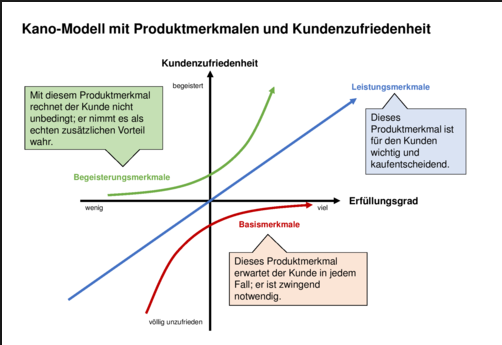
\includegraphics{res_qm/kanto.png}
    \end{field}
\end{note}

\begin{note}
    \xplain{Taylorismus - Erklärung}

    \bxplain{Mensch eine von aussen zu steuernde und kontrollierende „Kraftmaschine“. \\
            Nicht die Zuverlässigkeit und Leistungsfähigkeit einer Maschine erreicht. \\
            Menschen handelt tendenziell rational und ist rein ökonomisch motiviert. }
\end{note}

\begin{note}
    \xplain{Taylorismus - Nachteile}

    \begin{field}
        \begin{itemize}
            \item Trennung von Hand und Kopfarbeit
            \item Entfremdung zwischen Arbeiter und Produkt
            \item Demotivation
            \item Qualitätsmängel
            \item Verstärkung Qualitätskontrollen
        \end{itemize}
    \end{field}
\end{note}

\begin{note}
    \xplain{Vierzehn Managementprinzipien nach Deming (Demingsche Lehre)}

    \begin{field}
        \begin{itemize}
            \item Schafe den festen Willen zur ständigen Verbesserung im Unternehmen
            \item Schaffe ein Bewusstsein für Qualität
            \item Beseitige die Abhängigkeit von Vollkontrollen
            \item Richte dich nich tallein nach dem billigsten Angebot
            \item Verbressere ständig die Systeme
            \item Schaffe moderne Ausbildungsmethoden
            \item Sorge für richtiges Führungsverhalten
            \item Beseitige die Angst
            \item Beseitige Barrieren zwischen Geschäftsbereichen
            \item Setze postive Ziele statt negativer Kritik
            \item Betone die Qualität der Leistung, nicht die Quantität
            \item Ermögliche Stolz auf gute Arbeit
            \item Fördere Qualifikation und Weiterbildung
            \item Mache die ständige Verbesserung von Qualität und Produktivität zur Aufgabe der Unternehmensleistung
        \end{itemize}
    \end{field}
\end{note}

\begin{note}
    \xplain{Qualität heute}

    \begin{field}
        \begin{itemize}
            \item Gesetzliche Auflagen: Produkthaftung, Arbeitsplatzsicherheit, Umweltschutz
            \item Kundenerwartungen: steigende Qualitätsansprüche, Wertewandel, geändertes Konsumverhalten
            \item Verschärfter Wettbewerb: Globalisierung, gesättigte Märkte -> Kostendruck, Überkapazitäten
            \item Unternehmen: Shareholder Value, zunehmende Produktkomplexität, schnellere Markteinführung neuer Produkte
        \end{itemize}
    \end{field}
\end{note}

\end{document}
